\documentclass{brockcosc3p03}

% Figure placement control
\usepackage{float}    % provides the [H] placement specifier
\usepackage{placeins} % provides \FloatBarrier
% Math support
\usepackage{amsmath}
\usepackage{amssymb}
% Non-floating captions (for samepage compatibility)
\usepackage{capt-of}
% Hyperlink configuration
\usepackage{hyperref}
\hypersetup{hidelinks}

% TikZ for graph drawings
\usepackage{tikz}

\newcommand{\studentname}{Matt Keith}
\newcommand{\studentid}{6369664}
\newcommand{\assignnum}{4}

\begin{document}
\section*{Answer to Question 1}

\begin{table}[H]
\centering
\caption{Doctor Preferences}
\begin{tabular}{|c|c|c|c|}
\hline
\textbf{Doctor} & \textbf{1st Choice} & \textbf{2nd Choice} & \textbf{3rd Choice} \\
\hline
$X$ & $B$ & $A$ & $C$ \\
$Y$ & $A$ & $B$ & $C$ \\
$Z$ & $A$ & $B$ & $C$ \\
\hline
\end{tabular}
\end{table}

\begin{table}[H]
\centering
\caption{Hospital Preferences}
\begin{tabular}{|c|c|c|c|}
\hline
\textbf{Hospital} & \textbf{1st Choice} & \textbf{2nd Choice} & \textbf{3rd Choice} \\
\hline
$A$ & $X$ & $Y$ & $Z$ \\
$B$ & $Y$ & $X$ & $Z$ \\
$C$ & $X$ & $Y$ & $Z$ \\
\hline
\end{tabular}
\end{table}

\subsection*{(a)}

We run the Gale--Shapley algorithm step by step with hospitals proposing.

\textbf{Step 1:} Hospital $A$ proposes to $X$. Since $X$ is currently unmatched, $X$ tentatively accepts $A$.

Current tentative matching: $(A,X)$

\textbf{Step 2:} Hospital $B$ proposes to $Y$. Since $Y$ is currently unmatched, $Y$ tentatively accepts $B$.

Current tentative matching: $(A,X), (B,Y)$

\textbf{Step 3:} Hospital $C$ proposes to $X$. Doctor $X$ compares $C$ with the current match $A$. Since $X$ prefers $A$ to $C$, $X$ rejects $C$.

Current tentative matching: $(A,X), (B,Y)$

\textbf{Step 4:} Hospital $C$ proposes to $Y$. Doctor $Y$ compares $C$ with the current match $B$. Since $Y$ prefers $B$ to $C$, $Y$ rejects $C$.

Current tentative matching: $(A,X), (B,Y)$

\textbf{Step 5:} Hospital $C$ proposes to $Z$. Since $Z$ is currently unmatched, $Z$ tentatively accepts $C$.

Current tentative matching: $(A,X), (B,Y), (C,Z)$


Since all hospitals are now matched, the algorithm terminates. The resulting stable matching is
\[
(A,X),\ (B,Y),\ (C,Z).
\]

\subsection*{(b)}

To find another stable matching, we run the Gale--Shapley algorithm again, this time with doctors making the proposals.

\textbf{Step 1:} Doctor $X$ proposes to $B$. Since $B$ is currently unmatched, $B$ tentatively accepts $X$.

Current tentative matching: $(B,X)$

\textbf{Step 2:} Doctor $Y$ proposes to $A$. Since $A$ is currently unmatched, $A$ tentatively accepts $Y$.

Current tentative matching: $(A,Y), (B,X)$

\textbf{Step 3:} Doctor $Z$ proposes to $A$. Hospital $A$ compares $Z$ with the current match $Y$. Since $A$ prefers $Y$ to $Z$, $A$ rejects $Z$.

Current tentative matching: $(A,Y), (B,X)$

\textbf{Step 4:} Doctor $Z$ proposes to $B$. Hospital $B$ compares $Z$ with the current match $X$. Since $B$ prefers $X$ to $Z$, $B$ rejects $Z$.

Current tentative matching: $(A,Y), (B,X)$

\textbf{Step 5:} Doctor $Z$ proposes to $C$. Since $C$ is currently unmatched, $C$ tentatively accepts $Z$.

Current tentative matching: $(A,Y), (B,X), (C,Z)$

Since all doctors are now matched, the algorithm terminates. This gives the second stable matching:
\[
(A,Y),\ (B,X),\ (C,Z).
\]

To see that no other stable matching exists, observe that hospital $C$ must be matched with doctor $Z$ in any stable matching. Note that doctor $Z$ is the last choice of every hospital ($A$, $B$, and $C$). Although $C$ prefers $X$ and $Y$ to $Z$, both $X$ and $Y$ prefer hospitals $A$ or $B$ over $C$. Therefore, if $C$ were matched with either $X$ or $Y$, that doctor together with a more preferred hospital would form a blocking pair. Hence $(C,Z)$ must appear in every stable matching.

Once $(C,Z)$ is fixed, the remaining hospitals and doctors are $\{A,B\}$ and $\{X,Y\}$. There are only two possible complete matchings on these remaining participants:
\[
(A,X),(B,Y)
\]
and
\[
(A,Y),(B,X).
\]
Both of these matchings are stable. Therefore, this instance has exactly two stable matchings:
\[
(A,X),\ (B,Y),\ (C,Z)
\]
and
\[
(A,Y),\ (B,X),\ (C,Z).
\]

\subsection*{(c)}

Let $\mathrm{best}(A)$ denote the highest-ranked feasible doctor on Hospital $A$'s preference list. We prove that the hospital-proposing Gale--Shapley algorithm matches $A$ with $\mathrm{best}(A)$.

Suppose for contradiction that hospital $A$ is not matched with $\mathrm{best}(A)$ by the algorithm. Since hospitals propose in order from highest-ranked to lowest-ranked doctor, hospital $A$ must eventually propose to $\mathrm{best}(A)$. If $A$ is not matched with $\mathrm{best}(A)$ at the end of the algorithm, then $\mathrm{best}(A)$ must reject $A$ at some point.

When a doctor rejects a hospital in the Gale--Shapley algorithm, that doctor is already holding, or later receives, a hospital that the doctor prefers more. Therefore, once $\mathrm{best}(A)$ rejects $A$, doctor $\mathrm{best}(A)$ can never again be matched with $A$ in any stable matching, because $\mathrm{best}(A)$ will always end up with some hospital that is preferred to $A$, and the pair consisting of that preferred hospital and $\mathrm{best}(A)$ would block any matching containing $(A,\mathrm{best}(A))$.

This contradicts the definition of $\mathrm{best}(A)$ as a feasible doctor for $A$, since feasibility means that there exists some stable matching in which $A$ is matched with $\mathrm{best}(A)$. Hence our assumption was false. Therefore, the Gale--Shapley algorithm must match hospital $A$ with $\mathrm{best}(A)$.

\subsection*{(d)}

Let $\mathrm{worst}(\alpha)$ denote the lowest-ranked feasible hospital on Doctor $\alpha$'s preference list. We prove that the hospital-proposing Gale--Shapley algorithm matches doctor $\alpha$ with $\mathrm{worst}(\alpha)$.

From part (c), the hospital-proposing Gale--Shapley algorithm matches every hospital with its highest-ranked feasible doctor. Therefore, among all stable matchings, the outcome produced by the algorithm is the most favorable one for the hospitals. In particular, there cannot exist another stable matching in which some hospital receives a doctor that it prefers more than the one assigned by the algorithm.

Now consider any doctor $\alpha$. Suppose, for contradiction, that in the Gale--Shapley matching doctor $\alpha$ is matched with a hospital $H$ that $\alpha$ prefers to $\mathrm{worst}(\alpha)$. Since $\mathrm{worst}(\alpha)$ is feasible, by definition there exists a stable matching in which doctor $\alpha$ is matched with $\mathrm{worst}(\alpha)$ instead.

Compare these two stable matchings. In the Gale--Shapley matching, hospital $H$ is matched with $\alpha$. In the other stable matching, $\alpha$ is matched with $\mathrm{worst}(\alpha)$, so hospital $H$ must be matched with some other doctor. For the new matching to remain stable, hospital $H$ would have to receive a doctor that it prefers at least as much as $\alpha$. This would mean that $H$ receives a doctor that it prefers more than the one assigned in the Gale--Shapley matching.

But this contradicts part (c), which showed that every hospital already receives its best feasible doctor in the hospital-proposing Gale--Shapley matching. Therefore our assumption is impossible.

Hence doctor $\alpha$ cannot be matched with any hospital better than $\mathrm{worst}(\alpha)$ in the hospital-proposing Gale--Shapley algorithm. Since $\mathrm{worst}(\alpha)$ is feasible, the algorithm must match doctor $\alpha$ with exactly $\mathrm{worst}(\alpha)$.

\subsection*{(e)}

Yes. If doctors make the proposals instead of hospitals, then the Gale--Shapley algorithm works in favor of the doctors. In general, the proposing side obtains its best feasible stable partner. We can see this directly in the given example by running the algorithm with doctors proposing.

\textbf{Step 1:} Doctor $X$ proposes to $B$. Since $B$ is currently unmatched, $B$ tentatively accepts $X$.

Current tentative matching: $(B,X)$

\textbf{Step 2:} Doctor $Y$ proposes to $A$. Since $A$ is currently unmatched, $A$ tentatively accepts $Y$.

Current tentative matching: $(A,Y), (B,X)$

\textbf{Step 3:} Doctor $Z$ proposes to $A$. Hospital $A$ compares $Z$ with the current match $Y$. Since $A$ prefers $Y$ to $Z$, $A$ rejects $Z$.

Current tentative matching: $(A,Y), (B,X)$

\textbf{Step 4:} Doctor $Z$ proposes to $B$. Hospital $B$ compares $Z$ with the current match $X$. Since $B$ prefers $X$ to $Z$, $B$ rejects $Z$.

Current tentative matching: $(A,Y), (B,X)$

\textbf{Step 5:} Doctor $Z$ proposes to $C$. Since $C$ is currently unmatched, $C$ tentatively accepts $Z$.

Current tentative matching: $(A,Y), (B,X), (C,Z)$

Since all doctors are now matched, the algorithm terminates with the stable matching
\[
(A,Y),\ (B,X),\ (C,Z).
\]

Now compare this with the hospital-proposing outcome from part (a):
\[
(A,X),\ (B,Y),\ (C,Z).
\]

Under doctor-proposing Gale--Shapley, doctor $X$ is matched with $B$, which is $X$'s first choice, and doctor $Y$ is matched with $A$, which is $Y$'s first choice. In the hospital-proposing matching, $X$ gets $A$ and $Y$ gets $B$, which are both worse for them. Doctor $Z$ is matched with $C$ in both cases. Therefore, in this example, changing the dynamic so that doctors propose does work to the doctors' advantage.

\newpage
\section*{Answer to Question 2.}

Before answering the subsections, we reproduce the given graph $G$ using TikZ.

\begin{figure}[H]
\centering
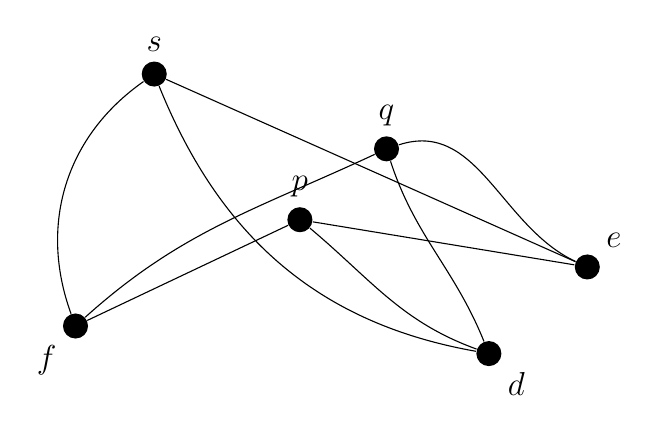
\begin{tikzpicture}[scale=1.0, every node/.style={font=\large}]
    % vertices
    \node[circle, fill=black, inner sep=3.2pt, label=above:$s$] (s) at (0.2,3.4) {};
    \node[circle, fill=black, inner sep=3.2pt, label=below left:$f$] (f) at (-0.8,0.2) {};
    \node[circle, fill=black, inner sep=3.2pt, label=above:$p$] (p) at (2.05,1.55) {};
    \node[circle, fill=black, inner sep=3.2pt, label=above:$q$] (q) at (3.15,2.45) {};
    \node[circle, fill=black, inner sep=3.2pt, label=below right:$d$] (d) at (4.45,-0.15) {};
    \node[circle, fill=black, inner sep=3.2pt, label=above right:$e$] (e) at (5.7,0.95) {};

    % edges
    \draw (s) to[out=215,in=110] (f);
    \draw (s) to[out=292,in=170] (d);
    \draw (s) to[out=336,in=156] (e);

    \draw (f) -- (p);
    \draw (f) to[out=42,in=205] (q);

    \draw (p) to[out=-40,in=160] (d);
    \draw (p) -- (e);

    \draw (q) to[out=-72,in=112] (d);
    \draw (q) to[out=18,in=155] (e);
\end{tikzpicture}
\caption{Graph $G$.}
\label{fig:q2-graph}
\end{figure}

\subsection*{(a)}

We execute the \textsc{Whatever-First-Search} algorithm starting from vertex $s$.
The bag initially contains only $(\varnothing,s)$.

\textbf{Step 1:} Remove $(\varnothing,s)$. Since $s$ is unmarked, mark $s$ and insert
$(s,v)$ for each neighbor $v$ of $s$.
The neighbors of $s$ are $f,d,e$, so the bag becomes
\[
\{(s,f),(s,d),(s,e)\}.
\]

\textbf{Step 2:} Remove $(s,f)$. Since $f$ is unmarked, mark $f$ and insert
$(f,v)$ for each neighbor $v$ of $f$.
The neighbors of $f$ are $s,p,q$, so the bag becomes
\[
\{(s,d),(s,e),(f,s),(f,p),(f,q)\}.
\]

\textbf{Step 3:} Remove $(f,p)$. Since $p$ is unmarked, mark $p$ and insert
$(p,v)$ for each neighbor $v$ of $p$.
The neighbors of $p$ are $f,d,e$, so the bag becomes
\[
\{(s,d),(s,e),(f,s),(f,q),(p,f),(p,d),(p,e)\}.
\]

\textbf{Step 4:} Remove $(p,d)$. Since $d$ is unmarked, mark $d$ and insert
$(d,v)$ for each neighbor $v$ of $d$.
The neighbors of $d$ are $s,p,q$, so the bag becomes
\[
\{(s,d),(s,e),(f,s),(f,q),(p,f),(p,e),(d,s),(d,p),(d,q)\}.
\]

\textbf{Step 5:} Remove $(d,q)$. Since $q$ is unmarked, mark $q$ and insert
$(q,v)$ for each neighbor $v$ of $q$.
The neighbors of $q$ are $f,d,e$, so the bag becomes
\[
\{(s,d),(s,e),(f,s),(f,q),(p,f),(p,e),(d,s),(d,p),(q,f),(q,d),(q,e)\}.
\]

\textbf{Step 6:} Remove $(q,e)$. Since $e$ is unmarked, mark $e$ and insert
$(e,v)$ for each neighbor $v$ of $e$.
The neighbors of $e$ are $s,p,q$, so the bag becomes
\[
\{(s,d),(s,e),(f,s),(f,q),(p,f),(p,e),(d,s),(d,p),(q,f),(q,d),(e,s),(e,p),(e,q)\}.
\]

At this point all vertices $s,f,p,d,q,e$ have been marked. The remaining
pairs correspond to already-marked vertices, so removing them causes no
further changes until the bag becomes empty.

\subsection*{(b)}
Breadth-First Search using a queue.

We execute the \textsc{Breadth-First-Search} algorithm starting from vertex $s$.
The bag is implemented as a queue (FIFO). The queue initially contains only $(\varnothing,s)$.
We represent the queue using square brackets. New pairs are inserted on the right side of the queue and removals occur from the left side.

\textbf{Step 1:} Remove $(\varnothing,s)$ from the front of the queue. Since $s$ is unmarked,
mark $s$ and insert $(s,v)$ for each neighbor $v$ of $s$.
The neighbors of $s$ are $f,d,e$, so the queue becomes
\[
[(s,f),(s,d),(s,e)].
\]

\textbf{Step 2:} Remove $(s,f)$. Since $f$ is unmarked, mark $f$ and insert
$(f,v)$ for each neighbor $v$ of $f$.
The neighbors of $f$ are $s,p,q$, so the queue becomes
\[
[(s,d),(s,e),(f,s),(f,p),(f,q)].
\]

\textbf{Step 3:} Remove $(s,d)$. Since $d$ is unmarked, mark $d$ and insert
$(d,v)$ for each neighbor $v$ of $d$.
The neighbors of $d$ are $s,p,q$, so the queue becomes
\[
[(s,e),(f,s),(f,p),(f,q),(d,s),(d,p),(d,q)].
\]

\textbf{Step 4:} Remove $(s,e)$. Since $e$ is unmarked, mark $e$ and insert
$(e,v)$ for each neighbor $v$ of $e$.
The neighbors of $e$ are $s,p,q$, so the queue becomes
\[
[(f,s),(f,p),(f,q),(d,s),(d,p),(d,q),(e,s),(e,p),(e,q)].
\]

\textbf{Step 5:} Remove $(f,s)$. Since $s$ is already marked, nothing happens.

\textbf{Step 6:} Remove $(f,p)$. Since $p$ is unmarked, mark $p$ and insert
$(p,v)$ for each neighbor $v$ of $p$.
The neighbors of $p$ are $f,d,e$, so the queue becomes
\[
[(f,q),(d,s),(d,p),(d,q),(e,s),(e,p),(e,q),(p,f),(p,d),(p,e)].
\]

\textbf{Step 7:} Remove $(f,q)$. Since $q$ is unmarked, mark $q$ and insert
$(q,v)$ for each neighbor $v$ of $q$.
The neighbors of $q$ are $f,d,e$, so the queue becomes
\[
[(d,s),(d,p),(d,q),(e,s),(e,p),(e,q),(p,f),(p,d),(p,e),(q,f),(q,d),(q,e)].
\]

At this point all vertices $s,f,d,e,p,q$ have been marked. The remaining
pairs correspond to already-marked vertices, so removing them causes no
further changes until the queue becomes empty.

\subsection*{(c)}
Iterative Depth-First Search using a stack.

We execute the \textsc{Iterative-Depth-First-Search} algorithm starting from
vertex $s$. The bag is implemented as a stack (LIFO). The stack initially contains only $(\varnothing,s)$.
We represent the stack using square brackets. Both insertion (push) and removal (pop) occur on the right side of the stack.

\textbf{Step 1:} Pop $(\varnothing,s)$. Since $s$ is unmarked, mark $s$ and push
$(s,v)$ for each neighbor $v$ of $s$.
The neighbors of $s$ are $f,d,e$, so the stack becomes
\[
[(s,f),(s,d),(s,e)].
\]

\textbf{Step 2:} Pop $(s,e)$. Since $e$ is unmarked, mark $e$ and push
$(e,v)$ for each neighbor $v$ of $e$.
The neighbors of $e$ are $s,p,q$, so the stack becomes
\[
[(s,f),(s,d),(e,s),(e,p),(e,q)].
\]

\textbf{Step 3:} Pop $(e,q)$. Since $q$ is unmarked, mark $q$ and push
$(q,v)$ for each neighbor $v$ of $q$.
The neighbors of $q$ are $f,d,e$, so the stack becomes
\[
[(s,f),(s,d),(e,s),(e,p),(q,f),(q,d),(q,e)].
\]

\textbf{Step 4:} Pop $(q,e)$. Since $e$ is already marked, nothing happens.

\textbf{Step 5:} Pop $(q,d)$. Since $d$ is unmarked, mark $d$ and push
$(d,v)$ for each neighbor $v$ of $d$.
The neighbors of $d$ are $s,p,q$, so the stack becomes
\[
[(s,f),(s,d),(e,s),(e,p),(q,f),(d,s),(d,p),(d,q)].
\]

\textbf{Step 6:} Pop $(d,q)$. Since $q$ is already marked, nothing happens.

\textbf{Step 7:} Pop $(d,p)$. Since $p$ is unmarked, mark $p$ and push
$(p,v)$ for each neighbor $v$ of $p$.
The neighbors of $p$ are $f,d,e$, so the stack becomes
\[
[(s,f),(s,d),(e,s),(e,p),(q,f),(d,s),(p,f),(p,d),(p,e)].
\]

\textbf{Step 8:} Pop $(p,e)$. Since $e$ is already marked, nothing happens.

\textbf{Step 9:} Pop $(p,d)$. Since $d$ is already marked, nothing happens.

\textbf{Step 10:} Pop $(p,f)$. Since $f$ is unmarked, mark $f$ and push
$(f,v)$ for each neighbor $v$ of $f$.
The neighbors of $f$ are $s,p,q$, so the stack becomes
\[
[(s,f),(s,d),(e,s),(e,p),(q,f),(d,s),(f,s),(f,p),(f,q)].
\]

At this point all vertices $s,e,q,d,p,f$ have been marked. Removing the
remaining pairs causes no further changes until the stack becomes empty.

\newpage
\section*{Answer to Question 3.}

% --- Begin Question 3 Graph Figure ---
\begin{figure}[H]
\centering
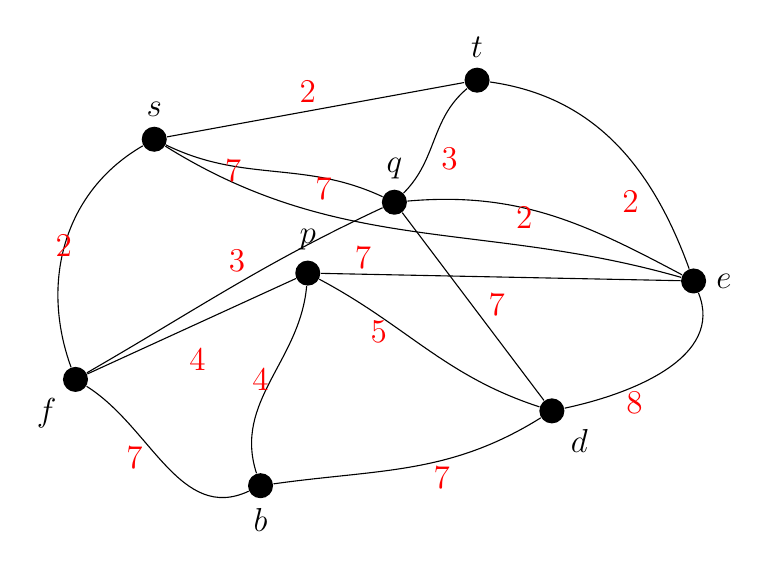
\begin{tikzpicture}[scale=1.0, every node/.style={font=\large}]
    % vertices
    \node[circle, fill=black, inner sep=3.2pt, label=above:$s$] (s) at (0.1,3.35) {};
    \node[circle, fill=black, inner sep=3.2pt, label=below left:$f$] (f) at (-0.9,0.3) {};
    \node[circle, fill=black, inner sep=3.2pt, label=above:$p$] (p) at (2.05,1.65) {};
    \node[circle, fill=black, inner sep=3.2pt, label=above:$q$] (q) at (3.15,2.55) {};
    \node[circle, fill=black, inner sep=3.2pt, label=above:$t$] (t) at (4.2,4.1) {};
    \node[circle, fill=black, inner sep=3.2pt, label=right:$e$] (e) at (6.95,1.55) {};
    \node[circle, fill=black, inner sep=3.2pt, label=below right:$d$] (d) at (5.15,-0.1) {};
    \node[circle, fill=black, inner sep=3.2pt, label=below:$b$] (b) at (1.45,-1.05) {};

    % edges
    \draw (s) -- (t);
    \draw (s) to[out=210,in=110] (f);
    \draw (s) to[out=328,in=164] (e);
    \draw (s) to[out=334,in=155] (q);

    \draw (f) to[out=30,in=205] (q);
    \draw (f) -- (p);
    \draw (f) to[out=-32,in=205] (b);

    \draw (p) -- (e);
    \draw (p) to[out=-95,in=108] (b);
    \draw (p) to[out=-28,in=162] (d);

    \draw (b) to[out=8,in=212] (d);

    \draw (q) to[out=45,in=220] (t);
    \draw (q) to[out=5,in=152] (e);
    \draw (q) -- (d);

    \draw (t) to[out=-8,in=110] (e);

    \draw (d) to[out=12,in=-68] (e);

    % manually placed weights
    \node[text=red] at (2.05,3.95) {2};   % s-t
    \node[text=red] at (-1.05,2.0) {2};   % s-f
    \node[text=red] at (1.10,2.95) {7};   % s-e
    \node[text=red] at (2.25,2.72) {7};   % s-q
    \node[text=red] at (1.15,1.8) {3};    % f-q
    \node[text=red] at (0.65,0.55) {4};   % f-p
    \node[text=red] at (-0.15,-0.7) {7};  % f-b
    \node[text=red] at (2.75,1.85) {7};   % p-e
    \node[text=red] at (1.45,0.3) {4};    % p-b
    \node[text=red] at (2.95,0.9) {5};    % p-d
    \node[text=red] at (3.75,-0.95) {7};  % b-d
    \node[text=red] at (3.85,3.1) {3};    % q-t
    \node[text=red] at (4.8,2.35) {2};    % q-e
    \node[text=red] at (4.45,1.25) {7};   % q-d
    \node[text=red] at (6.15,2.55) {2};   % t-e
    \node[text=red] at (6.2,0.0) {8};     % d-e

\end{tikzpicture}
\caption{Graph $G_{mst}$.}
\label{fig:q3-graph}
\end{figure}
% --- End Question 3 Graph Figure ---

\subsection*{(a)}

Using Kruskal's algorithm, we sort the edges of $G_{mst}$ by nondecreasing weight and add an edge whenever it does not create a cycle.

The edges in increasing order of weight are:
\[
2: \ st,\ sf,\ qe,\ te
\]
\[
3: \ fq,\ qt
\]
\[
4: \ fp,\ pb
\]
\[
5: \ pd
\]
\[
7: \ sq,\ se,\ fb,\ pe,\ bd,\ qd
\]
\[
8: \ de
\]

Now we apply Kruskal's algorithm step by step.

\textbf{Step 1:} Add $st$ (weight $2$).

\textbf{Step 2:} Add $sf$ (weight $2$).

\textbf{Step 3:} Add $qe$ (weight $2$).

\textbf{Step 4:} Add $te$ (weight $2$).

At this point the vertices $s,t,f,q,e$ are all in the same connected component.

\textbf{Step 5:} Consider $fq$ (weight $3$). Since $f$ and $q$ are already in the same component, adding $fq$ would create a cycle, so we skip it.

\textbf{Step 6:} Consider $qt$ (weight $3$). Since $q$ and $t$ are already in the same component, adding $qt$ would create a cycle, so we skip it.

\textbf{Step 7:} Add $fp$ (weight $4$).

\textbf{Step 8:} Add $pb$ (weight $4$).

\textbf{Step 9:} Add $pd$ (weight $5$).

Now the tree contains $7$ edges and all $8$ vertices are connected, so we have obtained an MST. Therefore,
\[
T_k = \{st,\ sf,\ qe,\ te,\ fp,\ pb,\ pd\}.
\]
The total weight is
\[
2+2+2+2+4+4+5 = 21.
\]

\subsection*{(b)}

Using Jarn\'ik's (Prim's) algorithm, we start from vertex $s$ and repeatedly add the minimum-weight edge with exactly one endpoint in the current tree.

\textbf{Step 1:} Start with the tree containing only $s$.

\textbf{Step 2:} One minimum-weight edge leaving $s$ is $sf$ of weight $2$. We choose $sf$ and add it to the tree.

\textbf{Step 3:} The minimum edge leaving $\{s,f\}$ is $st$ of weight $2$. Add $st$.

\textbf{Step 4:} The minimum edge leaving $\{s,f,t\}$ is $te$ of weight $2$. Add $te$.

\textbf{Step 5:} The minimum edge leaving $\{s,f,t,e\}$ is $eq$ of weight $2$. Add $eq$.

\textbf{Step 6:} The minimum edge leaving $\{s,f,t,e,q\}$ is $fp$ of weight $4$. Add $fp$.

\textbf{Step 7:} The minimum edge leaving $\{s,f,t,e,q,p\}$ is $pb$ of weight $4$. Add $pb$.

\textbf{Step 8:} The minimum edge leaving $\{s,f,t,e,q,p,b\}$ is $pd$ of weight $5$. Add $pd$.

Now all vertices are in the tree, so
\[
T_p = \{sf,\ st,\ te,\ eq,\ fp,\ pb,\ pd\}.
\]
The total weight is again
\[
2+2+2+2+4+4+5 = 21.
\]

\subsection*{(c)}

Yes. The two trees are the same, since they contain exactly the same set of edges from the original graph:
\[
T_k = T_p = \{st,\ sf,\ qe,\ te,\ fp,\ pb,\ pd\}.
\]
So Kruskal's algorithm and Jarn\'ik's (Prim's) algorithm produce the same MST for this graph.



\newpage
\section*{Answer to Question 4.}

\subsection*{(a)}

We create a graph $G_{unique}$ with four vertices and distinct edge weights so that the minimum spanning tree is unique.

\begin{figure}[H]
\centering
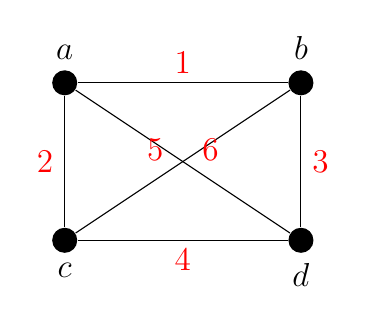
\begin{tikzpicture}[scale=1.0, every node/.style={font=\large}]
    % vertices
    \node[circle, fill=black, inner sep=3.2pt, label=above:$a$] (a) at (0,2) {};
    \node[circle, fill=black, inner sep=3.2pt, label=above:$b$] (b) at (3,2) {};
    \node[circle, fill=black, inner sep=3.2pt, label=below:$c$] (c) at (0,0) {};
    \node[circle, fill=black, inner sep=3.2pt, label=below:$d$] (d) at (3,0) {};

    % edges
    \draw (a) -- (b);
    \draw (a) -- (c);
    \draw (b) -- (d);
    \draw (c) -- (d);
    \draw (a) -- (d);
    \draw (b) -- (c);

    % weights
    \node[text=red] at (1.5,2.25) {1};
    \node[text=red] at (-0.25,1.0) {2};
    \node[text=red] at (3.25,1.0) {3};
    \node[text=red] at (1.5,-0.25) {4};
    \node[text=red] at (1.15,1.15) {5};
    \node[text=red] at (1.85,1.15) {6};
\end{tikzpicture}
\caption{A graph $G_{unique}$ with distinct edge weights.}
\label{fig:gunique}
\end{figure}

The unique MST is obtained by choosing the three smallest edges that connect all four vertices without creating a cycle. Therefore, the MST is
\[
T = \{ab, ac, bd\}.
\]
Its total weight is
\[
1 + 2 + 3 = 6.
\]

We can also illustrate the MST separately:

\begin{figure}[H]
\centering
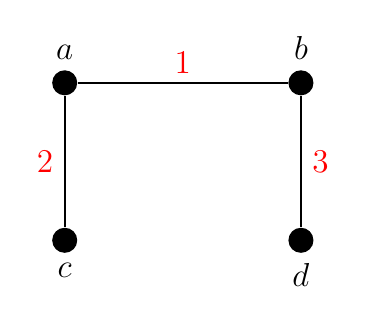
\begin{tikzpicture}[scale=1.0, every node/.style={font=\large}]
    % vertices
    \node[circle, fill=black, inner sep=3.2pt, label=above:$a$] (a) at (0,2) {};
    \node[circle, fill=black, inner sep=3.2pt, label=above:$b$] (b) at (3,2) {};
    \node[circle, fill=black, inner sep=3.2pt, label=below:$c$] (c) at (0,0) {};
    \node[circle, fill=black, inner sep=3.2pt, label=below:$d$] (d) at (3,0) {};

    % MST edges
    \draw[thick] (a) -- (b);
    \draw[thick] (a) -- (c);
    \draw[thick] (b) -- (d);

    % weights
    \node[text=red] at (1.5,2.25) {1};
    \node[text=red] at (-0.25,1.0) {2};
    \node[text=red] at (3.25,1.0) {3};
\end{tikzpicture}

\caption{The unique minimum spanning tree of $G_{unique}$.}
\label{fig:gunique-mst}
\end{figure}

\subsection*{(b)}

We prove that if a graph has unique edge weights, then it has a unique minimum spanning tree.

Suppose, for contradiction, that a graph $G$ has no repeated edge weights, but has two different minimum spanning trees, say $T_1$ and $T_2$.

Since $T_1$ and $T_2$ are different, there must be some edge that is in one tree but not the other. Let $e$ be the smallest-weight edge that appears in exactly one of the two trees. Without loss of generality, assume that $e \in T_1$ but $e \notin T_2$.

Now add $e$ to $T_2$. Since $T_2$ is already a spanning tree, adding one extra edge creates exactly one cycle. That cycle must contain some edge $f$ that is not in $T_1$, because $e$ is in the cycle and $e \notin T_2$.

By the choice of $e$, every edge of smaller weight is either in both trees or in neither tree. Since $f$ is another edge where the two trees differ, and $e$ was chosen to be the smallest such edge, we must have
\[
w(e) < w(f).
\]
This is where the assumption of unique edge weights matters: the weights cannot be equal.

If we remove $f$ from $T_2 \cup \{e\}$, we get another spanning tree. Its total weight is smaller than the total weight of $T_2$, because we removed the heavier edge $f$ and replaced it with the lighter edge $e$.

But this is impossible, since $T_2$ was assumed to be a minimum spanning tree.

Therefore, our assumption was false. So a graph with unique edge weights must have a unique minimum spanning tree.

\subsection*{(c)}

Yes, Dijkstra's algorithm produces a tree if we record for each vertex the edge through which it was first reached with minimum distance from the source \cite{bari_dijkstra}. This resulting tree is called a \emph{shortest-path tree}. However, it is not necessarily a minimum spanning tree.
The reason is that Dijkstra's algorithm and MST algorithms are solving different problems. Dijkstra's algorithm tries to minimize the distance from one chosen source vertex to every other vertex. In contrast, an MST tries to minimize the total weight of all edges in the tree. Those are different goals, so the resulting trees do not always match.

Here is a simple example. Consider the graph below, with source vertex $s$.

\begin{figure}[H]
\centering
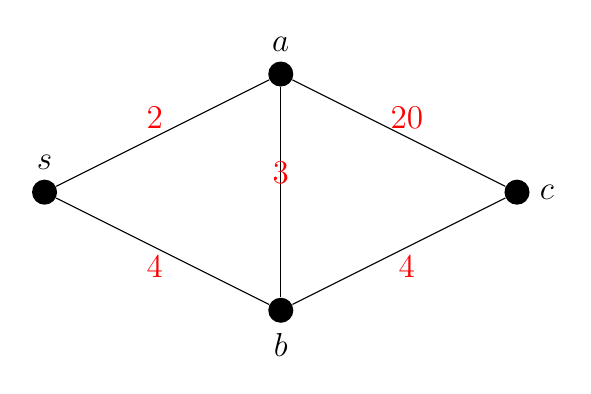
\begin{tikzpicture}[scale=1.0, every node/.style={font=\large}]
    % vertices
    \node[circle, fill=black, inner sep=3.2pt, label=above:$s$] (s) at (0,1.5) {};
    \node[circle, fill=black, inner sep=3.2pt, label=above:$a$] (a) at (3,3) {};
    \node[circle, fill=black, inner sep=3.2pt, label=below:$b$] (b) at (3,0) {};
    \node[circle, fill=black, inner sep=3.2pt, label=right:$c$] (c) at (6,1.5) {};

    % edges
    \draw (s) -- (a);
    \draw (s) -- (b);
    \draw (a) -- (c);
    \draw (b) -- (c);
    \draw (a) -- (b);

    % weights
    \node[text=red] at (1.4,2.45) {2};
    \node[text=red] at (1.4,0.55) {4};
    \node[text=red] at (4.6,2.45) {20};
    \node[text=red] at (4.6,0.55) {4};
    \node[text=red] at (3,1.75) {3};
\end{tikzpicture}
\caption{A graph where the shortest-path tree and the MST are different.}
\label{fig:q4c-example}
\end{figure}

If we run Dijkstra's algorithm from source $s$, we get:
\[
d(s,a)=2, \qquad d(s,b)=4, \qquad d(s,c)=8.
\]
The direct edge $sb$ has weight $4$, while the alternative path $s \to a \to b$ has weight $2+3=5$, so Dijkstra chooses $sb$ rather than going through $a$ when reaching $b$. Therefore one shortest-path tree is
\[
T_D = \{sa,\ sb,\ bc\}.
\]
This tree has total weight
\[
2+4+4=10.
\]

We can draw this shortest-path tree separately as follows:

\begin{figure}[H]
\centering
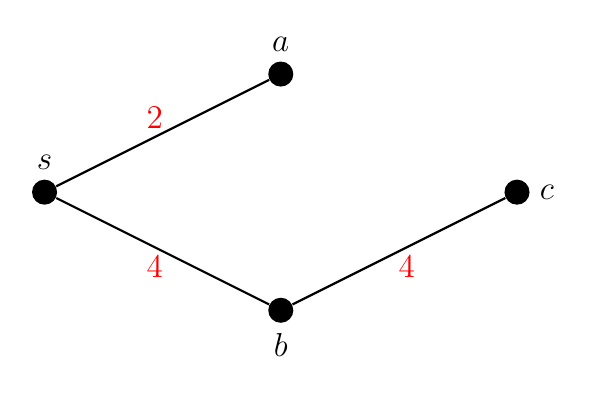
\begin{tikzpicture}[scale=1.0, every node/.style={font=\large}]
    % vertices
    \node[circle, fill=black, inner sep=3.2pt, label=above:$s$] (s) at (0,1.5) {};
    \node[circle, fill=black, inner sep=3.2pt, label=above:$a$] (a) at (3,3) {};
    \node[circle, fill=black, inner sep=3.2pt, label=below:$b$] (b) at (3,0) {};
    \node[circle, fill=black, inner sep=3.2pt, label=right:$c$] (c) at (6,1.5) {};

    % shortest-path tree edges
    \draw[thick] (s) -- (a);
    \draw[thick] (s) -- (b);
    \draw[thick] (b) -- (c);

    % weights
    \node[text=red] at (1.4,2.45) {2};
    \node[text=red] at (1.4,0.55) {4};
    \node[text=red] at (4.6,0.55) {4};
\end{tikzpicture}
\caption{The shortest-path tree produced by Dijkstra's algorithm from source $s$.}
\label{fig:q4c-dijkstra-tree}
\end{figure}

Now consider the MST of the same graph. An MST is obtained by choosing the edges
\[
ab,\ sa,\ bc.
\]
So an MST is
\[
T_M = \{ab,\ sa,\ bc\}.
\]
Its total weight is
\[
3+2+4=9.
\]

We can also draw the MST separately:

\begin{figure}[H]
\centering
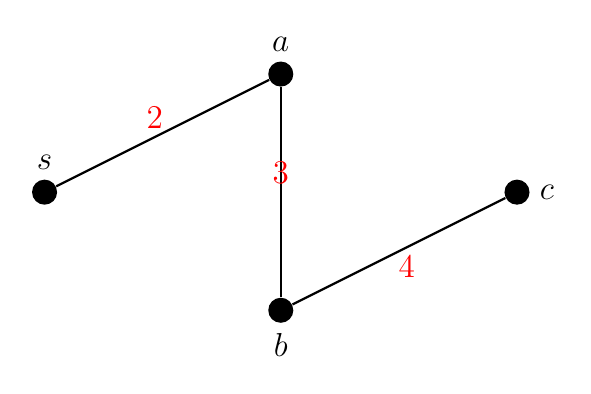
\begin{tikzpicture}[scale=1.0, every node/.style={font=\large}]
    % vertices
    \node[circle, fill=black, inner sep=3.2pt, label=above:$s$] (s) at (0,1.5) {};
    \node[circle, fill=black, inner sep=3.2pt, label=above:$a$] (a) at (3,3) {};
    \node[circle, fill=black, inner sep=3.2pt, label=below:$b$] (b) at (3,0) {};
    \node[circle, fill=black, inner sep=3.2pt, label=right:$c$] (c) at (6,1.5) {};

    % MST edges
    \draw[thick] (a) -- (b);
    \draw[thick] (s) -- (a);
    \draw[thick] (b) -- (c);

    % weights
    \node[text=red] at (3,1.75) {3};
    \node[text=red] at (1.4,2.45) {2};
    \node[text=red] at (4.6,0.55) {4};
\end{tikzpicture}
\caption{A minimum spanning tree of the same graph.}
\label{fig:q4c-mst-tree}
\end{figure}

Therefore, Dijkstra's algorithm does produce a tree, but in general it is a shortest-path tree, not a minimum spanning tree. In this example,
\[
T_D = \{sa,\ sb,\ bc\}
\]
and
\[
T_M = \{ab,\ sa,\ bc\},
\]
so the two trees are different.

In some graphs, the shortest-path tree and the MST may happen to be the same. For example, if a graph has edges
\[
sa=1,\quad sb=2,\quad ab=1,\quad bc=2,\quad ac=10,
\]
then one shortest-path tree from $s$ is $\{sa,ab,bc\}$, and this is also an MST. However, as the example above shows, Dijkstra's algorithm does not guarantee that this will happen.

\newpage

\section*{Answer to Question 5.}

\subsection*{(a)}

Memoization is a technique where we store the answers to recursive subproblems after computing them once, so that if the same subproblem appears again we can reuse the stored result instead of recomputing it. In this approach we still write the algorithm recursively, but we remember previously solved subproblems so that repeated work is avoided. This is often described as a \emph{top-down} approach.

\subsection*{(b)}

A subsequence is a sequence of characters that appears in the same relative order as in the original string, but not necessarily next to each other.

For example, in the string
\[
\texttt{ABCDE}
\]
the sequence
\[
\texttt{ACE}
\]
is a subsequence, because we keep the order $A \to C \to E$, even though the letters are not consecutive.

A substring is different because the characters must be consecutive. For example,
\[
\texttt{BCD}
\]
is a substring of \texttt{ABCDE}, but
\[
\texttt{ACE}
\]
is not a substring.

So the difference is:
\begin{itemize}
    \item a \textbf{subsequence} keeps the same order, but may skip characters;
    \item a \textbf{substring} must be a continuous block of characters.
\end{itemize}

\subsection*{(c)}

Let
\[
X = \texttt{ABFFSDERW}
\]
and
\[
Y = \texttt{WFDFTRESAWE}.
\]

We use dynamic programming. Let $L[i,j]$ denote the length of the LCS of the first $i$ characters of $X$ and the first $j$ characters of $Y$.

The dynamic programming rule for filling the table is:
\[
\text{if } X_i = Y_j, \text{ then } L[i,j] = 1 + L[i-1,j-1]
\]
\[
\text{else } L[i,j] = \max\{L[i-1,j], L[i,j-1]\}
\]
This is the same if/else rule used in Abdul Bari's explanation of LCS \cite{bari_lcs}.

Filling in the dynamic programming table gives the following values. The row numbers $1$ through $9$ correspond to the letters of $X=\texttt{ABFFSDERW}$, and the column numbers $1$ through $11$ correspond to the letters of $Y=\texttt{WFDFTRESAWE}$:

\[
\begin{array}{cc|cccccccccccc}
 & & 0 & 1 & 2 & 3 & 4 & 5 & 6 & 7 & 8 & 9 & 10 & 11 \\
 & & \varnothing & W & F & D & F & T & R & E & S & A & W & E \\
\hline
0 & \varnothing & 0 & 0 & 0 & 0 & 0 & 0 & 0 & 0 & 0 & 0 & 0 & 0 \\
1 & A & 0 & 0 & 0 & 0 & 0 & 0 & 0 & 0 & 0 & 1 & 1 & 1 \\
2 & B & 0 & 0 & 0 & 0 & 0 & 0 & 0 & 0 & 0 & 1 & 1 & 1 \\
3 & F & 0 & 0 & 1 & 1 & 1 & 1 & 1 & 1 & 1 & 1 & 1 & 1 \\
4 & F & 0 & 0 & 1 & 1 & 2 & 2 & 2 & 2 & 2 & 2 & 2 & 2 \\
5 & S & 0 & 0 & 1 & 1 & 2 & 2 & 2 & 2 & 3 & 3 & 3 & 3 \\
6 & D & 0 & 0 & 1 & 2 & 2 & 2 & 2 & 2 & 3 & 3 & 3 & 3 \\
7 & E & 0 & 0 & 1 & 2 & 2 & 2 & 2 & 3 & 3 & 3 & 3 & 4 \\
8 & R & 0 & 0 & 1 & 2 & 2 & 2 & 3 & 3 & 3 & 3 & 3 & 4 \\
9 & W & 0 & 1 & 1 & 2 & 2 & 2 & 3 & 3 & 3 & 3 & 4 & 4 \\
\end{array}
\]

The final entry is $L[9,11] = 4$, so the length of the LCS is 4.

To recover an actual longest common subsequence, we backtrack from the bottom-right corner of the table.

Starting at $(9,11)$, which is the bottom-right corner of the table (row $W$, column $E$), the value is $4$. Since the last characters are $W$ and $E$, they do not match, so we move to a neighboring cell with the same value. Moving left takes us to $(9,10)$, where the characters are $W$ and $W$, so they match. Therefore, $W$ is part of an LCS, and we move diagonally to $(8,9)$.

At $(8,9)$, the characters are $R$ and $A$, so they do not match. We again move to a neighboring cell with the same value. Continuing this process and recording matched characters eventually produces one longest common subsequence.

During backtracking it can happen that the cell above and the cell to the left have the same value. When this occurs, we may move in either direction without changing the LCS length. For example, from a cell with value $3$ we might move left several times (left–left–left) or move up several times (up–up–up) as long as the values remain the same. Each different sequence of choices can lead to a different longest common subsequence.

Because of these ties in the table, the LCS is not unique in this example. One valid backtracking path gives $\texttt{FDEW}$, but other valid backtracking choices produce different longest common subsequences of the same length.

For example, some longest common subsequences are
\[
\texttt{FDEW},\quad \texttt{FDRW},\quad \texttt{FFEW},\quad \texttt{FFRW},\quad \texttt{FFSE},\quad \texttt{FFSW}.
\]
Each of these subsequences has length
\[
\boxed{4}.
\]

\newpage
\bibliographystyle{unsrt}
\bibliography{books}
\end{document}
